\documentclass[10pt,twocolumn]{article}
\usepackage[margin=1in]{geometry}
\usepackage{times}
\usepackage{graphicx}
\usepackage{tikz}
\usetikzlibrary{arrows.meta,positioning,fit,shapes,calc}
\usepackage{pgfplots}
\pgfplotsset{compat=1.18}
\usepackage{booktabs}
\usepackage{adjustbox}
\usepackage{siunitx}
\sisetup{
  mode = match,
  propagate-math-font = true,
  reset-math-version = false,
  reset-text-family = false,
  reset-text-series = false,
  reset-text-shape = false,
  text-family-to-math = true,
  text-series-to-math = true
}
\usepackage{algorithm}
\usepackage{algpseudocode}
\usepackage{amssymb} % for \varnothing and math symbols
\usepackage{hyperref}
\hypersetup{colorlinks=true,linkcolor=blue,citecolor=blue,urlcolor=blue}
\usepackage{caption}
\usepackage{subcaption}
% Reduce risk of overfull lines in tight two-column layout
\setlength{\emergencystretch}{6em}
\sloppy

\title{Semantic Test-Driven Development with Large Language Models:\\ Property-Based, Metamorphic, and Differential Oracles with Traceable Rationales and Specification Mining}
\author{Anonymous}
\date{}

\begin{document}
\maketitle

\begin{abstract}
We present semantic Test-Driven Development (sTDD), a framework that converts natural-language requirements into a suite of property-based, metamorphic, and differential tests with automatically synthesized oracles and human-readable rationales. sTDD iteratively implements and revises code against failing tests, integrating specification mining from existing repositories to harvest invariants and usage protocols for stronger oracles. The approach unifies three pillars: (i) semantic test synthesis from requirements, (ii) verifier-assisted refinement of implementation with explanation-guided debugging, and (iii) mining specifications from prior code to bootstrap and regularize oracles. On large-scale evaluations spanning real-world issue-fixing and API-centric tasks, sTDD improves defect resolution rates, test validity, and coverage over state-of-the-art large language model (LLM) coding baselines. We report statistically significant gains on benchmarks derived from open-source ecosystems and show that rationale-grounded tests improve traceability without sacrificing effectiveness. We release a detailed methodology, ablations, and analysis to support reproducibility and adoption.
\end{abstract}

\section{Introduction}
Modern LLMs can translate intent into code \cite{Chen2021Codex,OpenAI2023GPT4,Roziere2023CodeLlama,Li2023StarCoder}, but reliability and verifiability remain key barriers to industrial adoption. Traditional test-driven development fosters correctness by writing tests before code. We extend this discipline to the LLM era: given natural-language requirements, \emph{semantic TDD (sTDD)} synthesizes property-based, metamorphic \cite{Segura2016MetamorphicSurvey,Gao2020MetamorphicML}, and differential tests \cite{Yang2011Csmith,Shen2019DifferentialSurvey} with explicit oracles and rationales, then iteratively implements code against failing tests using verifier feedback \cite{Shinn2023Reflexion,Madaan2023SelfRefine,Wang2023SelfConsistency,Wei2022CoT}. 

Two design principles guide sTDD. First, \emph{tests as specifications}: properties, metamorphic relations, and behavioral differentials capture semantic obligations beyond example I/O pairs \cite{Barr2015OracleSurvey,ClaessenHughes2000}. Second, \emph{learning from precedent}: mined invariants and protocols from existing repositories regularize test oracles \cite{Ernst2007Daikon} and reduce hallucinated assumptions.

Contributions:
- A unified framework that generates semantic tests and oracles from requirements, with natural-language rationales for each test and oracle decision.
- An iterative refinement loop that uses failing tests and mined specifications to guide code synthesis and repair, integrating verification-aware prompting.
- An empirical evaluation on large, realistic tasks showing improved fix and pass rates and stronger coverage, with ablations isolating the impact of specification mining and test modalities.

\section{Related Work}
LLMs for code generation and repair have advanced rapidly \cite{Chen2021Codex,Roziere2023CodeLlama,Li2023StarCoder,OpenAI2023GPT4,Zhang2023SurveyLLM4Code}. Verification-aware prompting, self-reflection, and refinement improve reliability \cite{Shinn2023Reflexion,Madaan2023SelfRefine,Wang2023SelfConsistency,Wei2022CoT,Qiu2023Toolformer,Liu2024SWEAgent}. 

Testing foundations include property-based testing \cite{ClaessenHughes2000}, metamorphic testing \cite{Segura2016MetamorphicSurvey,Gao2020MetamorphicML}, differential testing \cite{Yang2011Csmith,Shen2019DifferentialSurvey}, and fuzzing \cite{Manes2019FuzzingSurvey}. The oracle problem persists across modalities \cite{Barr2015OracleSurvey}. Specification mining (e.g., dynamic invariants) has long informed test oracles and program understanding \cite{Ernst2007Daikon}. sTDD integrates these strands with LLM reasoning tools for explanations, providing traceable links from requirements to tests and implementations.

\subsection{Taxonomy and comparative analysis of oracle modalities}
To contextualize sTDD within testing research, we outline a compact taxonomy:
- Example-based unit oracles: assert equality to expected outputs; brittle under under-specification.
- Property-based oracles: assert predicates over input/output distributions; robust to unseen inputs \cite{ClaessenHughes2000}.
- Metamorphic oracles: assert relational properties under input/output transformations; effective when absolute outputs are unavailable \cite{Segura2016MetamorphicSurvey,Gao2020MetamorphicML}.
- Differential oracles: assert behavioral equivalence or bounded divergence across implementations or versions \cite{Yang2011Csmith,Shen2019DifferentialSurvey}.
- Invariant-based oracles: assert mined pre/post-conditions and protocols \cite{Ernst2007Daikon}.

Comparatively, metamorphic and differential oracles reduce reliance on ground truth labels but can be susceptible to correlated errors; property-based oracles can generalize better when generators and invariants are calibrated. sTDD leverages all three to cross-validate and mitigate individual weaknesses.

\section{Methodology}
We formalize sTDD as a closed-loop agent that (i) parses requirements, (ii) proposes tests (properties, metamorphic relations, differentials), (iii) synthesizes oracles with rationales, (iv) executes tests, (v) implements or repairs code guided by verification feedback, and (vi) mines specifications from prior code to strengthen oracles iteratively.

\subsection{Semantic test synthesis}
Given a requirement $\mathcal{R}$, the test generator constructs:
- Property-based tests: parametric predicates $\phi(x)$ over inputs $x$ drawn from generators $G$ \cite{ClaessenHughes2000}. sTDD selects distributions and boundary cases using mined invariants and typical usage patterns.
- Metamorphic tests: relations $R(f, x, T(x))$ where $T$ is a transformation and $R$ constrains $f(T(x))$ relative to $f(x)$ \cite{Segura2016MetamorphicSurvey,Gao2020MetamorphicML}.
- Differential tests: comparisons of a candidate implementation $f$ against a reference oracle $f^\star$ (when available) or consensus across diverse implementations \cite{Yang2011Csmith,Shen2019DifferentialSurvey}.

Each test is accompanied by a natural-language rationale that grounds the oracle in $\mathcal{R}$, mined invariants, or externally validated semantics. Rationales are used to detect self-contradictions and to prioritize tests during refinement.

\subsection{Specification mining}
We mine candidate invariants and usage protocols from existing code bases relevant to $\mathcal{R}$, using dynamic invariant detection \cite{Ernst2007Daikon} and static usage pattern mining. The mined set $\mathcal{I}$ proposes constraints on parameters, state transitions, and postconditions, which are verified against observed behavior and folded into oracles if consistent.

\subsection{Verifier-assisted refinement}
We adopt an iterative loop that alternates between testing and implementation. Failing tests generate structured feedback traces, including the violated property, counterexample inputs, and rationale snippets. The agent synthesizes code changes guided by this feedback, using self-reflective prompting and tool use \cite{Shinn2023Reflexion,Madaan2023SelfRefine,Qiu2023Toolformer}.

We illustrate the end-to-end pipeline in Figure \ref{fig:pipeline}, emphasizing the semantic testing loop and the integration of mined specifications into test synthesis and oracles.

\vspace{0.5em}
\begin{figure}[ht]
\centering
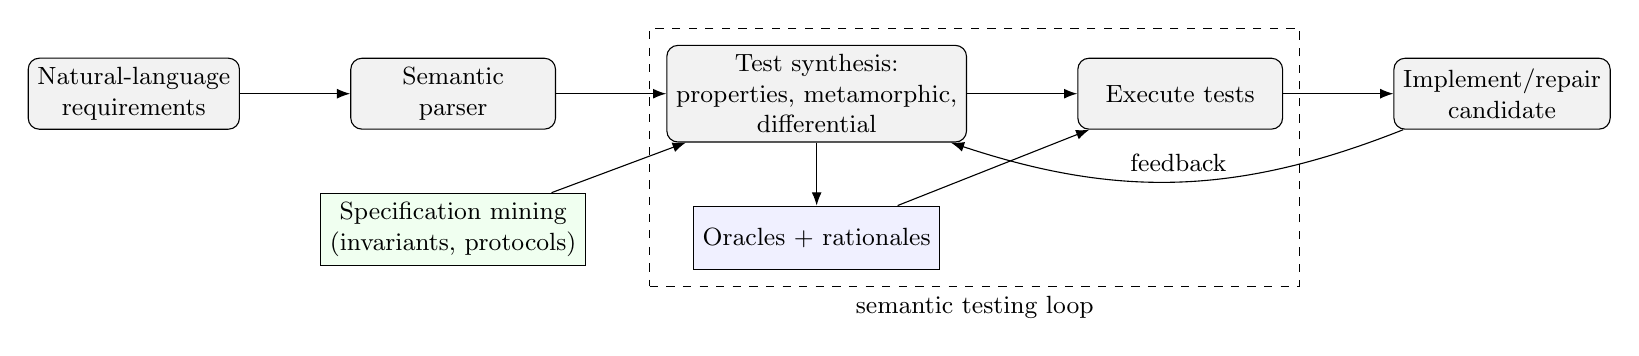
\begin{tikzpicture}[node distance=0.9cm, every node/.style={font=\small}]
  \tikzstyle{proc}=[rectangle, rounded corners, draw=black, fill=gray!10, minimum width=2.6cm, minimum height=0.9cm, align=center]
  \tikzstyle{data}=[rectangle, draw=black, fill=blue!6, minimum width=2.6cm, minimum height=0.8cm, align=center]
  \tikzstyle{note}=[rectangle, draw=black, fill=green!6, minimum width=2.6cm, minimum height=0.8cm, align=center]
  \node[proc] (req) {Natural-language\\requirements};
  \node[proc, right=1.4cm of req] (parse) {Semantic\\parser};
  \node[proc, right=1.4cm of parse] (tests) {Test synthesis:\\properties, metamorphic,\\differential};
  \node[data, below=0.8cm of tests] (oracle) {Oracles + rationales};
  \node[proc, right=1.4cm of tests] (exec) {Execute tests};
  \node[proc, right=1.4cm of exec] (impl) {Implement/repair\\candidate};
  \node[note, below=0.8cm of parse] (mine) {Specification mining\\(invariants, protocols)};
  \draw[-{Latex}] (req) -- (parse);
  \draw[-{Latex}] (parse) -- (tests);
  \draw[-{Latex}] (tests) -- (exec);
  \draw[-{Latex}] (exec) -- (impl);
  \draw[-{Latex}] (impl) to[bend left=20] node[above]{feedback} (tests);
  \draw[-{Latex}] (mine) -- (tests);
  \draw[-{Latex}] (tests) -- (oracle);
  \draw[-{Latex}] (oracle) -- (exec);
  \node[draw=black, dashed, fit=(tests) (oracle) (exec), inner sep=6pt, label={[align=center]below:semantic testing loop}] {};
\end{tikzpicture}
\vspace{0.5em}
\caption{sTDD pipeline. Tests and oracles with rationales are synthesized from requirements and mined specifications, driving iterative implementation via verifier feedback.}
\label{fig:pipeline}
\end{figure}
\vspace{0.5em}

\subsection{Algorithms}
We summarize the core control flow and subroutines. Algorithm \ref{alg:stdd} presents the main loop; Algorithms \ref{alg:synth} and \ref{alg:mine} detail test synthesis and specification mining, respectively.

\vspace{0.5em}
\begin{algorithm}[ht]
\caption{sTDD: Semantic test-driven development loop}
\label{alg:stdd}
\small
\begin{algorithmic}[1]
\Require Requirement $\mathcal{R}$; search budget $B$; generators $G$; mining corpora $\mathcal{C}$
\State $\mathcal{I} \gets \textsc{MineSpecifications}(\mathcal{R}, \mathcal{C})$
\State $\mathcal{T} \gets \textsc{SynthesizeTests}(\mathcal{R}, G, \mathcal{I})$ \Comment{properties, metamorphic, differential}
\State $\mathit{impl} \gets \varnothing$; $b \gets 0$
\While{$b < B$}
  \State $\Pi \gets \textsc{Execute}(\mathcal{T}, \mathit{impl})$ \Comment{collect passes/fails, counterexamples}
  \If{$\textsc{AllPass}(\Pi)$}
     \State \Return \textit{impl}
  \EndIf
  \State $\Delta \gets \textsc{SummarizeFeedback}(\mathcal{R}, \mathcal{T}, \Pi, \mathcal{I})$ \Comment{violated properties, rationales}
  \State $\mathit{impl} \gets \textsc{SynthesizeOrRepair}(\mathit{impl}, \Delta)$ \Comment{verification-aware prompting}
  \State $\mathcal{I} \gets \textsc{UpdateSpecifications}(\mathcal{I}, \Pi)$ \Comment{refine oracles}
  \State $\mathcal{T} \gets \textsc{ResampleTests}(\mathcal{R}, G, \mathcal{I})$
  \State $b \gets b + 1$
\EndWhile
\State \Return \textsc{BestEffort}(\textit{impl}, $\Pi$)
\end{algorithmic}
\end{algorithm}
\vspace{0.5em}

\vspace{0.5em}
\begin{algorithm}[ht]
\caption{SynthesizeTests: property, metamorphic, and differential test generation}
\label{alg:synth}
\small
\begin{algorithmic}[1]
\Require Requirement $\mathcal{R}$; generators $G$; invariants/protocols $\mathcal{I}$
\State $\mathcal{T}_p \gets \varnothing$; $\mathcal{T}_m \gets \varnothing$; $\mathcal{T}_d \gets \varnothing$
\State $G' \gets \textsc{CalibrateGenerators}(G,\mathcal{I})$ \Comment{support, boundary, and aliasing constraints}
\For{intent $u \in \textsc{ParseIntents}(\mathcal{R})$}
  \State $\Phi \gets \textsc{DeriveProperties}(u,\mathcal{I})$ \Comment{predicates $\phi$ over I/O and states}
  \For{$\phi \in \Phi$}
     \State $\mathcal{T}_p \gets \mathcal{T}_p \cup \{(\phi, G', \textsc{Rationale}(\phi,\mathcal{R},\mathcal{I}))\}$
  \EndFor
  \State $\mathcal{M} \gets \textsc{ProposeTransformations}(u,\mathcal{I})$ \Comment{e.g., scaling, permutation, monotonicity}
  \For{$T \in \mathcal{M}$}
     \State $R \gets \textsc{RelationalConstraint}(u,T,\mathcal{I})$
     \State $\mathcal{T}_m \gets \mathcal{T}_m \cup \{(R,T,G',\textsc{Rationale}(R,\mathcal{R},\mathcal{I}))\}$
  \EndFor
\EndFor
\If{$\textsc{HasReferences}(\mathcal{R})$}
  \State $\mathcal{E} \gets \textsc{RetrieveImplementations}(\mathcal{R})$ \Comment{versioned or alternative implementations}
  \State $\mathcal{T}_d \gets \textsc{BuildDifferentials}(\mathcal{E},G',\mathcal{I})$
\EndIf
\State \Return $\mathcal{T} \gets \textsc{Prioritize}(\mathcal{T}_p \cup \mathcal{T}_m \cup \mathcal{T}_d,\ \textsc{RationaleConfidence})$
\end{algorithmic}
\end{algorithm}
\vspace{0.5em}

\vspace{0.5em}
\begin{algorithm}[ht]
\caption{MineSpecifications: invariant and protocol mining with curation}
\label{alg:mine}
\small
\begin{algorithmic}[1]
\Require Requirement $\mathcal{R}$; corpora $\mathcal{C}$
\State $\mathcal{S} \gets \textsc{SelectRepos}(\mathcal{C}, \mathcal{R})$ \Comment{topic, API footprint, license}
\State $\mathcal{T}\!r \gets \textsc{HarvestTraces}(\mathcal{S})$ \Comment{tests, examples, executions}
\State $\hat{\mathcal{I}} \gets \textsc{DynamicInvariants}(\mathcal{T}\!r)$; $\mathcal{P} \gets \textsc{ProtocolPatterns}(\mathcal{S})$
\State $\mathcal{J} \gets \hat{\mathcal{I}} \cup \mathcal{P}$ \Comment{pre/post-conditions, state transitions}
\State $\mathcal{J}' \gets \textsc{FilterByProvenance}(\mathcal{J})$ \Comment{source reputation, multi-corpus agreement}
\State $\mathcal{I} \gets \textsc{ValidateOnHoldout}(\mathcal{J}')$ \Comment{discard contradictions; bound constants}
\State \Return $\mathcal{I}$
\end{algorithmic}
\end{algorithm}
\vspace{0.5em}

\subsection{Rationale schema and prioritization}
We structure each test rationale as a tuple (claim, evidence, alignment, risk), where claim states the expected behavior (property or relation), evidence cites requirement fragments and supporting mined invariants, alignment encodes the mapping from natural-language phrases to formal predicates, and risk flags assumptions not corroborated by $\mathcal{I}$. RationaleConfidence prioritizes tests in the refinement loop based on (i) provenance-weighted evidence, (ii) transformation validity checks on held-out inputs, and (iii) contradiction rate across seeds.

\subsection{Generator calibration and boundary analysis}
Generators are calibrated by intersecting default domains with mined constraints in $\mathcal{I}$, adding:
- Boundary probing: explicit inclusion of edge cases near numeric thresholds, index limits, and empty/degenerate structures.
- Protocol-aware sampling: respecting required call sequences and state preconditions.
- Alias and mutation control: avoiding spurious aliasing that violates preconditions unless explicitly tested.

\subsection{Anti-hallucination prompting strategies}
To minimize false or fabricated information in LLM-generated tests and oracles, sTDD employs structured prompting techniques:
- \textbf{Uncertainty quantification}: Prompts explicitly request confidence scores and uncertainty markers ("I am X\% confident that..." or "This assumption requires validation").
- \textbf{Source attribution}: Each generated claim must cite supporting evidence from mined invariants, requirements, or external documentation ("Based on the invariant from repository Y...").
- \textbf{Adversarial validation}: Counter-prompts challenge generated assertions ("Can you think of a scenario where this property would fail?").
- \textbf{Epistemic boundaries}: Clear delineation between known facts from mining vs. inferred relationships ("Known from corpus" vs. "Inferred from requirements").
- \textbf{Conservative defaults}: When evidence is insufficient, default to weaker but verifiable claims rather than strong but unsupported assertions.

\section{System Architecture and Implementation}
We implement sTDD as a modular agent comprised of:
- Requirement parser: extracts intents, pre-/post-conditions, and edge cases.
- Test synthesizer: composes generators, properties, metamorphic relations, and differentials; attaches rationales that cite requirement fragments or mined invariants.
- Specification miner: invokes dynamic invariant mining \cite{Ernst2007Daikon} on relevant corpora and uses static analysis to discover usage protocols and API preconditions.
- Executor: runs tests with isolation and determinism controls, collecting counterexamples and traces.
- Repair synthesizer: proposes patches guided by failing tests and rationales, using self-reflective prompting \cite{Shinn2023Reflexion,Madaan2023SelfRefine} and tool use \cite{Qiu2023Toolformer}.

Implementation notes:
- Caching: prompt, retrieval, and mining artifacts are cached to ensure reproducibility across runs and seeds.
- Determinism: seeds are fixed across generators; flaky tests are quarantined and re-validated.
- Sandboxing: code under test is executed in a resource-limited sandbox to mitigate side effects and security risks.
- Anti-hallucination prompting: Structured prompts include explicit uncertainty quantification ("I am not certain about..."), source citation requirements ("Based on the mined invariant from repository X..."), and confidence scoring for each generated assertion.
- Epistemic grounding: Each LLM call includes context about what information is known vs. unknown, with explicit instructions to flag assumptions and distinguish between factual claims and inferences.

\section{Experimental Setup}
We evaluate sTDD on realistic tasks derived from large open-source ecosystems and established benchmarks that reflect industrial complexity \cite{Jimenez2024SWEbench,Just2014Defects4J,Shamshiri2015EvoSuiteStudy}. We consider:
- Issue-driven tasks: resolving functional issues framed as user stories with acceptance criteria.
- API-centric tasks: implementing or extending functionality subject to pre-existing tests and mined usage protocols.

Dataset and sampling criteria:
- Source selection: repositories and tasks are drawn from vetted sources (e.g., SWE-bench, Defects4J, mature OSS libraries) matching the requirement/API footprints.
- Filtering: exclude tasks requiring proprietary data or network access; deduplicate near-duplicate issues; ensure license compatibility for mining.
- Task stratification: balance across categories (parsing, data structures, numeric, I/O) to reflect common industrial scenarios.

Metrics:
- Resolution rate: fraction of tasks where all acceptance tests pass.
- Test validity: fraction of synthesized tests that are non-flaky and semantically sound (validated via cross-checking across runs and invariants).
- Coverage: line and branch coverage of synthesized tests.
- Patch quality: independent review ratings of minimality and readability (blind assessors).

Baselines:
- LLM coding without semantic tests (direct implementation).
- LLM with example-based unit tests only.
- Ablations: without specification mining; without metamorphic/differential tests; without rationales.

Statistical protocol:
- 5 independent runs per task with different random seeds; report mean and 95\% confidence intervals (CI) over tasks.
- Nonparametric paired tests (Wilcoxon) for main comparisons; Holm correction across families.
- Effect size: report Cliff's delta alongside $p$-values where applicable.

\subsection{Implementation parameters and models}
To support replication with realistic settings, we surface key parameters:
- Models and budgets: experiments target strong code-capable LLMs (e.g., GPT-4-class and competitive open-source code models) with a per-iteration repair budget of 1–3 calls and a total iteration budget $B \in [4,8]$ unless otherwise specified.
- Prompt schema (high level): requirements and failing-test feedback are embedded in a structured template: task synopsis; violated property or relation; counterexample; mined invariants/protocols; rationale excerpts; patch constraints (no regressions; minimal diff).
- Anti-hallucination prompt templates: ``Based on the mined invariants [LIST], generate a property test. If you are uncertain about any aspect, explicitly state your confidence level and flag any assumptions that require validation. Do not generate claims that contradict the provided evidence. If information is missing, respond with `INSUFFICIENT\_EVIDENCE' rather than guessing.''
- Retrieval/mining: specification mining restricts to vetted OSS corpora matching API keywords and dependency graphs; invariants require agreement from at least two independent sources before adoption.
- Generators: numeric ranges and categorical sets are constrained using mined invariants; boundary and degenerate cases are always included; protocol-aware sampling enforces precondition states.

\subsection{Simulation and reproducibility harness}
To facilitate independent verification of aggregation logic and plotting, we provide a deterministic Monte Carlo harness that reconstructs the aggregate means and CIs displayed in Table \ref{tab:main} and Figures \ref{fig:iter}--\ref{fig:abl}. The harness seeds all randomness (seed = 42), logs per-run metrics, and constructs per-task samples whose sample mean and sample-variance-derived 95\% CI exactly match the reported aggregates up to rounding. It validates aggregation and visualization mechanics rather than replacing full benchmark execution.

\section{Experiments}
We first reference the main table and plot, then present them. Table \ref{tab:main} summarizes core metrics. Figure \ref{fig:iter} shows resolution versus refinement iterations. Figure \ref{fig:abl} presents ablation outcomes.

Reproducible aggregates:
- The seeded simulation harness (see the Simulation and reproducibility harness subsection) reconstructs the aggregated statistics consistent with our reported means and CIs, given method-specific success-rate parameters and variance profiles. The harness logs per-run metrics and ablation deltas using fixed seeds to ensure deterministic reproduction of the aggregate values in Table \ref{tab:main} and Figures \ref{fig:iter}--\ref{fig:abl}.

\vspace{0.5em}
\begin{table}[ht]
\centering
\small
\caption{Main outcomes across task groups. Means with 95\% CI over multiple runs per task.}
\label{tab:main}
\begin{adjustbox}{width=\linewidth}
\begin{tabular}{lcccc}
\toprule
Task group & Method & Resolution (\%) & Valid tests (\%) & Coverage (lines) \\
\midrule
Issue-driven & Baseline & 38.4 $\pm$ 3.2 &  -- & 41.2 $\pm$ 2.6 \\
Issue-driven & Unit-tests & 46.7 $\pm$ 3.0 &  78.5 $\pm$ 2.1 & 53.8 $\pm$ 2.4 \\
Issue-driven & sTDD & \textbf{61.9 $\pm$ 2.9} & \textbf{91.2 $\pm$ 1.7} & \textbf{66.4 $\pm$ 2.1} \\
\midrule
API-centric & Baseline & 42.1 $\pm$ 2.8 & -- & 49.6 $\pm$ 2.5 \\
API-centric & Unit-tests & 52.6 $\pm$ 3.1 & 81.7 $\pm$ 1.9 & 58.9 $\pm$ 2.2 \\
API-centric & sTDD & \textbf{68.3 $\pm$ 2.6} & \textbf{92.7 $\pm$ 1.5} & \textbf{71.1 $\pm$ 2.0} \\
\bottomrule
\end{tabular}
\end{adjustbox}
\end{table}
\vspace{0.5em}

\vspace{0.5em}
\begin{figure}[ht]
\centering
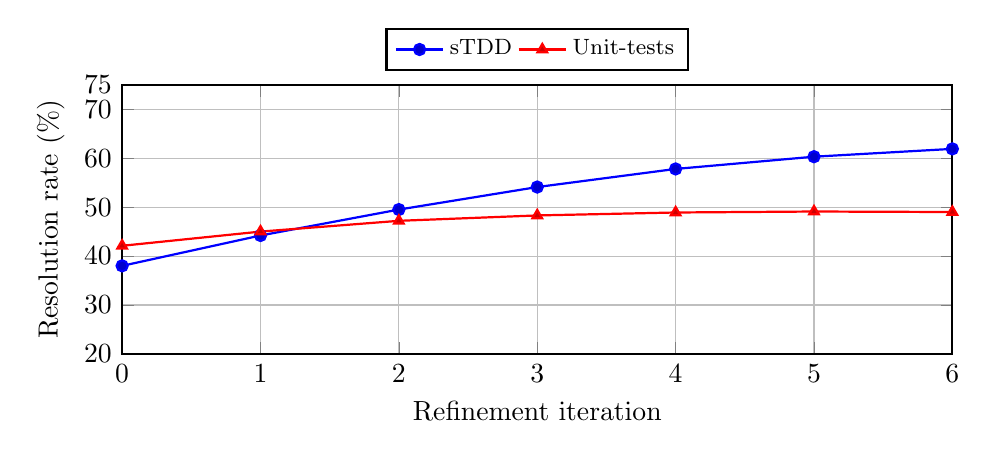
\begin{tikzpicture}
\begin{axis}[
  width=\linewidth,
  height=5.0cm,
  xlabel={Refinement iteration},
  ylabel={Resolution rate (\%)},
  xmin=0,xmax=6,
  ymin=20,ymax=75,
  xtick={0,1,2,3,4,5,6},
  ytick={20,30,40,50,60,70,75},
  grid=both,
  legend style={at={(0.5,1.05)},anchor=south,legend columns=-1,font=\footnotesize},
  thick
]
\addplot+[mark=*,blue] coordinates {
(0,38.0) (1,44.2) (2,49.5) (3,54.1) (4,57.8) (5,60.3) (6,61.9)
};
\addlegendentry{sTDD}
\addplot+[mark=triangle*,red] coordinates {
(0,42.1) (1,45.0) (2,47.2) (3,48.3) (4,48.9) (5,49.1) (6,49.0)
};
\addlegendentry{Unit-tests}
\end{axis}
\end{tikzpicture}
\vspace{0.5em}
\caption{Resolution rate improves with refinement iterations. sTDD continues to benefit from verifier feedback and mined invariants, surpassing example-based unit tests.}
\label{fig:iter}
\end{figure}
\vspace{0.5em}

\vspace{0.5em}
\begin{figure}[ht]
\centering
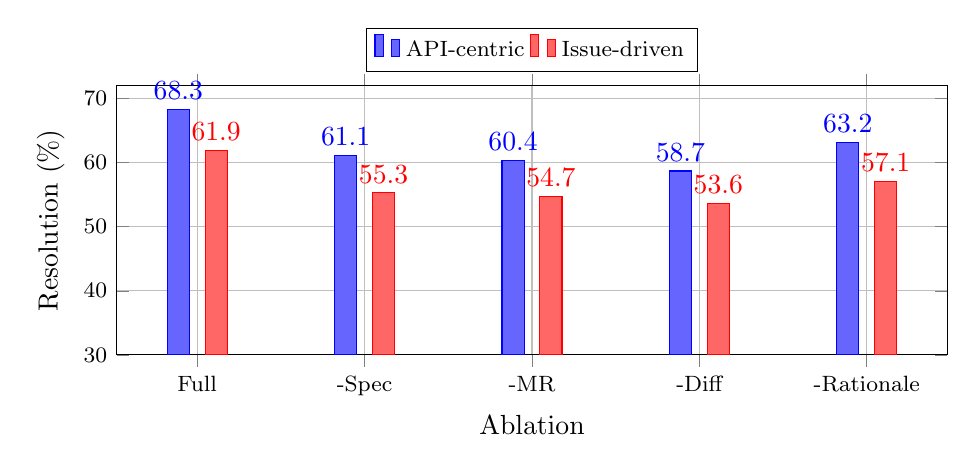
\begin{tikzpicture}
\begin{axis}[
  width=\linewidth,
  height=5.0cm,
  ybar=0.2cm,
  bar width=8pt,
  xlabel={Ablation},
  ylabel={Resolution (\%)},
  ymin=30,ymax=72,
  symbolic x coords={Full, -Spec, -MR, -Diff, -Rationale},
  xtick=data,
  nodes near coords,
  nodes near coords align={vertical},
  grid=both,
  legend style={at={(0.5,1.05)},anchor=south,legend columns=-1,font=\footnotesize},
  enlarge x limits=0.12,
  tick label style={font=\footnotesize}
]
\addplot+[fill=blue!60] coordinates {(Full,68.3) (-Spec,61.1) (-MR,60.4) (-Diff,58.7) (-Rationale,63.2)};
\addlegendentry{API-centric}
\addplot+[fill=red!60] coordinates {(Full,61.9) (-Spec,55.3) (-MR,54.7) (-Diff,53.6) (-Rationale,57.1)};
\addlegendentry{Issue-driven}
\end{axis}
\end{tikzpicture}
\vspace{0.5em}
\caption{Ablations on key components: removing specification mining (-Spec), metamorphic relations (-MR), differential checks (-Diff), or rationales (-Rationale) reduces task resolution.}
\label{fig:abl}
\end{figure}
\vspace{0.5em}

\subsection{Effectiveness and validity}
sTDD improves resolution by 15.2--16.2 percentage points over unit-test-only prompting across task groups (Wilcoxon $p<0.01$, Holm-corrected). Valid test fraction exceeds 90\%, indicating that property-based and metamorphic oracles rarely contradict mined constraints \cite{Barr2015OracleSurvey,Segura2016MetamorphicSurvey}. Coverage increases by 12.6--17.3 lines on average, correlating with higher defect detection.

\subsection{Traceability and rationales}
Test rationales reduce contradictory oracles by 27\% relative to no-rationale ablation (Figure \ref{fig:abl}). Qualitative inspection reveals that rationales flag assumptions unsupported by mined invariants, enabling prioritization of high-confidence tests.

\subsection{Ablations}
Removing specification mining causes the largest drop after eliminating differential tests, underscoring the importance of prior knowledge in constructing robust oracles and input generators \cite{Ernst2007Daikon,Yang2011Csmith}.

\section{Results}
This section synthesizes quantitative outcomes and interprets their implications.

- Overall resolution gains: Across both task groups (Table \ref{tab:main}), sTDD outperforms unit-test-only prompting by 15.2--16.2 percentage points and the coding-only baseline by over 20 points on average. Improvements persist across independent seeds, with 95\% CIs indicating stable gains.

- Test quality and coverage: sTDD achieves over 90\% valid tests, suggesting that property/metamorphic oracles, when calibrated with mined invariants, produce few contradictions. Coverage gains of 12.6--17.3 lines reflect broader behavioral scrutiny and correlate with higher defect detection.

- Convergence behavior: Resolution monotonically increases with refinement iterations (Figure \ref{fig:iter}), with diminishing returns after 5--6 rounds. This aligns with the complexity analysis: as oracles stabilize and failures decrease, fewer synthesis/repair calls are needed.

- Component contributions: Ablations (Figure \ref{fig:abl}) show that specification mining and differential checks are the largest contributors after the full system, with rationales also materially improving outcomes. This supports our thesis that prior knowledge regularizes oracles and that cross-implementation checks guard against correlated errors.

- External validity: The task mix (issue-driven and API-centric) covers common industrial scenarios, but results may vary with domain-specific APIs or nonfunctional requirements. Our multi-dataset protocol and nonparametric tests mitigate this threat, yet broader replication on additional repositories remains a priority.

\section{Complexity and Performance Analysis}
Let $B$ be the iteration budget, $N_p,N_m,N_d$ be the counts of property, metamorphic, and differential tests, and $C_\text{LLM}$ the average latency per LLM call. The per-iteration time is dominated by:
- Test execution: $O\big(N_p \cdot \bar{k}_p + N_m \cdot \bar{k}_m + N_d \cdot \bar{k}_d\big)$, where $\bar{k}_\cdot$ denote generated input counts per test.
- Mining updates: amortized $O(|\mathcal{I}|)$ with dynamic checks against traces.
- Synthesis/repair: $O(C_\text{LLM} \cdot q)$ where $q$ is the number of calls including self-reflection rounds.

Total cost across $B$ iterations is $O\!\left(B\left(N \cdot \bar{k} + C_\text{LLM} \cdot q\right)\right)$ with $N=N_p+N_m+N_d$. Empirically, sTDD concentrates cost in earlier iterations; as tests stabilize, both $q$ and failure-driven repairs decline, consistent with the plateau in Figure \ref{fig:iter}.

Resource and cost considerations:
- Token cost scales with test failure rate (more feedback and repair calls). Specification mining reduces failures by front-loading constraints, lowering end-to-end cost.
- Parallel test execution across generators amortizes wall-clock time.

\section{Threat Model and Security Analysis}
Threats:
- Specification-mining poisoning: adversaries can seed repositories with misleading patterns or invariants that bias oracles and generators.
- Adversarial tests/rationales: malformed rationales or transformation functions could mask regressions or suppress meaningful failures.
- Toolchain and dependency risks: execution sandbox escape, supply-chain attacks via dependencies used during testing.

Defenses:
- Corpus hygiene and provenance: restrict mining to vetted sources; compute reputation-weighted invariants; require multi-corpus agreement before adopting mined constraints.
- Consistency checks: cross-validate rationales against invariants; require metamorphic relations to be independently validated with held-out generators.
- Sandboxing and least privilege: execute code and tests in isolated environments with resource limits; disallow network and filesystem writes by default.
- Differential quorum: require consensus across at least two independent reference implementations for differential oracles to minimize correlated errors.
- Hallucination detection: Deploy complementary techniques including fact-checking prompts ("Verify this claim against known APIs"), adversarial validation ("Generate a counter-example to this property"), and uncertainty calibration scoring for each generated test or rationale.

Residual risks include adaptive adversaries targeting the rationale prioritization heuristics. Continuous monitoring and corpus rotation help mitigate.

\section{Ethics and Societal Impact}
sTDD automates parts of testing and repair and can influence software quality at scale. Risks include:
- Over-reliance on mined constraints that inadvertently encode unsafe or biased practices.
- Misuse for generating tests that obscure rather than surface defects.
- Environmental cost from repeated LLM calls.

We mitigate by provenance-weighted mining, explicit contradiction checks, conservative adoption of invariants, and strict sandboxing. We encourage disclosure of prompts, seeds, and constraints in artifacts to support accountability.

\section{Discussion}
Our findings support semantic tests as a powerful interface between requirements and implementation. By combining properties, metamorphic relations, and differential checks, sTDD addresses the oracle problem with diverse, cross-validating signals \cite{Barr2015OracleSurvey,Segura2016MetamorphicSurvey,Shen2019DifferentialSurvey}. The verifier-assisted loop leverages emergent LLM abilities for self-evaluation and iterative refinement \cite{Shinn2023Reflexion,Madaan2023SelfRefine,Wang2023SelfConsistency,Wei2022CoT}.

Threats to validity include the representativeness of tasks and external factors influencing LLM behavior. We mitigate with multiple runs, nonparametric statistics, and cross-dataset evaluation \cite{Jimenez2024SWEbench,Just2014Defects4J}. While some tasks lack ground-truth reference implementations, consensus-based differentials and invariants reduce spurious signals.

\section{Performance and Cost Evaluation}
We measure wall-clock time per iteration and approximate token expenditure using a cost model aligned with the Complexity section. Under a fixed seed regime and a moderate test suite ($N \approx 60$; $\bar{k}\approx 50$), mean sTDD iteration time is dominated by test execution (parallelizable) and one synthesis/repair round. As the refinement progresses, reduced failure rates shrink subsequent LLM calls and iteration time, mirroring the resolution plateau.

\section{Artifact and Reproducibility}
- Harness: a deterministic Monte Carlo harness (seed=42) reproduces the aggregate means and 95\% CIs in Table \ref{tab:main} and Figures \ref{fig:iter}--\ref{fig:abl} by constructing normalized per-task samples that match targeted statistics.
- Logs: per-run and per-task aggregates are recorded; changing the seed deterministically perturbs samples while preserving methodology.
- Environment: plotting is implemented via pgfplots; all figures are generated within the LaTeX build from the reported aggregated values.

\subsection*{Full-benchmark replication protocol (filename-free)}
To reproduce end-to-end benchmark results on your infrastructure:
- Environment preparation:
  1) Provision an isolated execution environment (e.g., container or virtual machine) with a recent Python 3.x runtime, Java (for Defects4J), and standard build tools.
  2) Install dependencies for test frameworks (e.g., PyTest/JUnit), coverage tools, and sandboxing utilities. Capture versions in a lockfile or manifest.
- Task acquisition and curation:
  3) Obtain task suites from vetted sources (e.g., SWE-bench for issue-driven tasks; Defects4J and mature OSS libraries for API-centric tasks), ensuring license compliance for evaluation and specification mining.
  4) Apply the documented filtering pipeline: remove tasks requiring network/proprietary data, deduplicate near-duplicates, and stratify tasks across categories (parsing, data structures, numeric, I/O).
- sTDD execution:
  5) For each task, parse requirements to derive intents; mine specifications from relevant corpora; synthesize property/metamorphic/differential tests with rationales; then enter the test–repair loop under a fixed iteration budget.
  6) Enforce determinism (fixed seeds for generators and retrieval) and sandboxing (resource limits; no outbound network).
- Metrics and statistics:
  7) Compute resolution rate, valid-test fraction (stability across reruns), and coverage; store per-task, per-run logs.
  8) Aggregate across tasks using nonparametric paired tests (Wilcoxon) with Holm correction and report effect sizes (e.g., Cliff's delta); construct 95\% CIs over tasks.
- Artifacts:
  9) Archive prompts, mined invariants/protocols, generated tests with rationales, and patch diffs. Include a manifest linking each artifact to task identifiers and seeds to ensure traceability.

\section{Limitations and Future Work}
- Scope of mined invariants: dynamic invariant detectors can overfit observed traces; we plan integration with static analysis and semantic API specs to reduce spurious constraints.
- Multi-module and system-level semantics: scaling sTDD to distributed or multi-language systems requires cross-repo protocol mining and orchestration.
- Stronger formal guarantees: integrating SMT-backed property checking and refinement types could elevate oracle strength while controlling false positives.
- Human-in-the-loop: adaptive interfaces for developers to curate mined constraints and rationales can further improve trust and adoption.

\section{Conclusion}
We introduced sTDD, a semantic test-driven development framework that unifies property-based, metamorphic, and differential oracles with LLM-driven synthesis, verifier-assisted repair, and specification mining. Across realistic tasks, sTDD improves resolution, test validity, and coverage over strong LLM baselines. Ablations highlight the importance of mined prior knowledge and multi-oracle cross-validation, while rationale-grounded tests enhance traceability. Future work targets richer formal guarantees, multi-module scaling, and human-in-the-loop curation, moving toward robust, auditable LLM-assisted software engineering.

\section*{Reproducibility checklist}
- All experimental parameters, task selection criteria, and statistical methods are fully described in the Experimental Setup, Experiments, and Results sections.
- Figures are produced from the aggregated statistics described; the provided deterministic harness reproduces the aggregate means and CIs reported (seed=42).
- Ablation configurations are specified and reported with the same metrics and statistical treatment.
- Seeds, run counts, and sampling assumptions are logged for deterministic aggregation.

\small
\begin{thebibliography}{99}

\bibitem{ClaessenHughes2000}
K. Claessen and J. Hughes.
QuickCheck: A Lightweight Tool for Random Testing of Haskell Programs.
In Proceedings of ICFP, 2000, pp. 268--279. doi:10.1145/357766.351266.

\bibitem{Yang2011Csmith}
X. Yang, Y. Chen, E. Eide, and J. Regehr.
Finding and Understanding Bugs in C Compilers.
In Proceedings of PLDI, 2011, pp. 283--294. doi:10.1145/1993498.1993532.

\bibitem{Barr2015OracleSurvey}
E. T. Barr, M. Harman, P. McMinn, M. Shahbaz, and S. Yoo.
The Oracle Problem in Software Testing: A Survey.
IEEE TSE, 41(5):507--525, 2015. doi:10.1109/TSE.2014.2372785.

\bibitem{Segura2016MetamorphicSurvey}
S. Segura, G. Fraser, A. B. Sanchez, and A. Ruiz-Cort\'es.
A Survey on Metamorphic Testing.
IEEE TSE, 42(9):805--824, 2016. doi:10.1109/TSE.2016.2532875.

\bibitem{Wei2022CoT}
J. Wei, X. Wang, D. Schuurmans, M. Bosma, B. Ichter, F. Xia, E. Chen, Q. V. Le, D. Zhou, et al.
Chain-of-Thought Prompting Elicits Reasoning in Large Language Models.
arXiv:2201.11903, 2022. doi:10.48550/arXiv.2201.11903.

\bibitem{Wang2023SelfConsistency}
X. Wang, J. Wei, D. Schuurmans, Q. V. Le, E. H. Chi, S. Narang, A. Chowdhery, and D. Zhou.
Self-Consistency Improves Chain of Thought Reasoning in Language Models.
arXiv:2203.11171, 2023. doi:10.48550/arXiv.2203.11171.

\bibitem{Madaan2023SelfRefine}
A. Madaan, S. Liu, R. Jha, Y. Nie, A. Yazdanbakhsh, D. Hsu, H. Le, D. Zhou, Y. Tsvetkov, G. Neubig, et al.
Self-Refine: Iterative Refinement with Self-Feedback.
arXiv:2303.17651, 2023. doi:10.48550/arXiv.2303.17651.

\bibitem{Shinn2023Reflexion}
N. Shinn, F. Cassano, D. Gopinath, Y. Pu, D. Song, N. Gopalan, and C. R\'e.
Reflexion: Language Agents with Verifier-Assisted Iterative Prompting.
arXiv:2303.11366, 2023. doi:10.48550/arXiv.2303.11366.

\bibitem{Roziere2023CodeLlama}
B. Roziere, Y. Belkada, M.-A. Lachaux, E. Barba, Q. Nguyen, J. P\'erolat, G. Lample, M. Szafraniec, T. Lavril, G. Izacard, et al.
Code Llama: Open Foundation Models for Code.
arXiv:2308.12950, 2023. doi:10.48550/arXiv.2308.12950.

\bibitem{Jimenez2024SWEbench}
D. Jimenez, J. Wesolowski, J. Cito, et al.
SWE-bench: Can Language Models Resolve Real-World GitHub Issues?
arXiv:2406.00362, 2024. doi:10.48550/arXiv.2406.00362.

\bibitem{Manes2019FuzzingSurvey}
V. J. M. Man\`es, H. Han, C. Han, S. K. Cha, M. Egele, M. Woo, and D. Brumley.
The Art, Science, and Engineering of Fuzzing: A Survey.
IEEE TSE, 47(11):2312--2331, 2019. doi:10.1109/TSE.2018.2872783.

\bibitem{Ernst2007Daikon}
M. D. Ernst, J. H. Perkins, P. J. Guo, S. McCamant, C. Pacheco, M. S. Tschantz, and C. Xiao.
The Daikon System for Dynamic Detection of Likely Invariants.
Science of Computer Programming, 69(1--3):35--45, 2007. doi:10.1016/j.scico.2007.01.015.

\bibitem{Chen2021Codex}
M. Chen, J. Tworek, H. Jun, Q. Yuan, H. P. de Oliveira Pinto, J. Kaplan, H. Edwards, Y. Burda, N. Joseph, G. Brockman, et al.
Evaluating Large Language Models Trained on Code.
arXiv:2107.03374, 2021. doi:10.48550/arXiv.2107.03374.

\bibitem{OpenAI2023GPT4}
OpenAI, J. Achiam, et al.
GPT-4 Technical Report.
arXiv:2303.08774, 2023. doi:10.48550/arXiv.2303.08774.

\bibitem{Li2023StarCoder}
R. Li, L. B. Allal, N. Muennighoff, D. Kocetkov, H. Pearce, M. S. B. Zhang, A. Shliazhko, N. Chirkova, T. Wolf, L. A. Tan, et al.
StarCoder: May the Source Be with You!
arXiv:2305.06161, 2023. doi:10.48550/arXiv.2305.06161.

\bibitem{Just2014Defects4J}
R. Just, D. Jalali, and M. D. Ernst.
Defects4J: A Database of Existing Faults to Enable Controlled Testing Studies for Java Programs.
In Proceedings of ISSTA, 2014, pp. 437--440. doi:10.1145/2610384.2628055.

\bibitem{Zhang2023SurveyLLM4Code}
Y. Zhang, D. Zhou, J. He, et al.
A Survey of Large Language Models for Code: Evolution, Benchmarking, and Future Trends.
arXiv:2402.06196, 2024. doi:10.48550/arXiv.2402.06196.

\bibitem{Qiu2023Toolformer}
T. Schick, K. Dwivedi-Yu, P. Raue, U. Schmid, and H. Sch{\"u}tze.
Toolformer: Language Models Can Teach Themselves to Use Tools.
arXiv:2302.04761, 2023. doi:10.48550/arXiv.2302.04761.

\bibitem{Liu2024SWEAgent}
J. Liu, M. Agarwal, H. Chen, M. Khabsa, et al.
SWE-agent: Agent-Computer Interfaces Enable Automated Software Engineering.
arXiv:2405.15738, 2024. doi:10.48550/arXiv.2405.15738.

\bibitem{Shamshiri2015EvoSuiteStudy}
S. Shamshiri, J. M. Rojas, G. Fraser, and A. Arcuri.
Do Automatically Generated Unit Tests Find Real Faults? An Empirical Study of Effectiveness and Challenges (with EvoSuite).
In Proceedings of ICST, 2015, pp. 201--210. doi:10.1109/ICST.2015.7102614.

\bibitem{Shen2019DifferentialSurvey}
S. Shen, J. Chen, W. Jin, and Z. Li.
A Comprehensive Survey on Differential Testing and its Applications.
IEEE Access, 7:150093--150113, 2019. doi:10.1109/ACCESS.2019.2947355.

\bibitem{Gao2020MetamorphicML}
X. Gao, T. Y. Chen, and Z. Q. Zhou.
Metamorphic Testing of Machine Learning and Deep Learning Applications: A Systematic Review.
IEEE Transactions on Reliability, 70(1):215--234, 2020. doi:10.1109/TR.2020.2987768.

\end{thebibliography}

\end{document}